\clearpage\nobalance
\section*{Author Notes}
\subsection*{Acknowledgements}
I thank Prof. Luyao Zhang, Program Chair, and Prof. Ken Rogerson, Program Discussant, of the \emph{2056 Nobel and Turing Laureate Program Launch Workshop}, held at Duke Kunshan University, IB 2050, on September 7, 2026. I also thank Mustafa Ayub Khan and Aaron Wang, my teammates in Session D, \emph{Strategic AI: Trust, Collusion, and Adaptation in Repeated Interactions}, and the rest of the COMSCI/ECON 206 Autumn 2026 Session 1 class for their questions and discussion. Preparing the Session D talk alongside their topics---sovereign disclosure and reliance on AI advice---is what pushed me to state the criterion at the level of reputation systems in general rather than payments alone. I am responsible for the proposal and remaining errors.

\subsection*{Individual contribution}
I designed the mechanism and its payoff structure, wrote and deployed the interactive game, ported the generator to Python and ran the sweep and ablation, verified both tool licences and the three anchor papers against their originals, produced the Draw.io teaser, and wrote the proposal. No code or text was shared with teammates; their contribution was discussion, acknowledged above. AI assistance is disclosed in Appendix~\ref{app:ai}.

\bibliographystyle{ACM-Reference-Format}\bibliography{references}
\appendix
\section{Technical details and reproducibility}
\label{app:tech}

\textbf{Artifacts.} Repository \url{https://github.com/ltishere/PS1-Tian} at commit \texttt{8172a7a}; notebook \texttt{notebook/coaching\_proof\_sweep.ipynb}; deployed game \url{https://dku-comsci-econ206-2026-tian-liang.static.hf.space/index.html}, served under the Hugging Face Static SDK with no server runtime, backend, database, secret or API call. Hosting, network transfer and the visitor's browser still consume resources; no claim of zero impact is made.

\textbf{Mechanism.} Twelve payment episodes per round. State: a credibility stock starting at 12 that never refills and carries across rounds, and a script rate starting at 0.50. Outcomes: fraud paid $-a$; a legitimate payment held $-0.3a$; a legitimate payment made $+0.01a$; a record query $-5$; a customer question $-1$ credibility.

\begin{table}[h]
\caption{Mechanism rules. The signal decides; the player chooses only which signal to read.}
\label{tab:rules}
\footnotesize
\begin{tabularx}{\columnwidth}{@{}lYl@{}}
\toprule
Mechanism & Signal read & Rule \\
\midrule
Pay now & none & always pay \\
Ask the customer & within-episode testimony & pay unless it conflicts \\
Check payee record & others' reports on the payee & pay unless flagged \\
Hold the payment & none & never pay \\
\bottomrule
\end{tabularx}
\end{table}

A coached payer's testimony never conflicts. An uncoached payer's probability of noticing is $0.75\times(\text{credibility}/12)$. The record flags a fraudulent payee with probability $p$ and a legitimate one with probability $0.05$. After each round the fraudster's script rate moves with the share of testimony checks it faced. Reset clears all state; nothing is written to storage, and the same seed with the same actions reproduces a round exactly.

\textbf{Notebook.} Python 3 with NumPy and Matplotlib only, both preinstalled in Colab; no external data, since every episode is generated from a seeded sequence. Runtime $\rightarrow$ Run all completes in roughly thirty seconds. The notebook follows predict $\rightarrow$ run $\rightarrow$ change one assumption $\rightarrow$ check $\rightarrow$ interpret, and states its three predictions before any cell executes.

\textbf{Recorded tests.} Run by hand in the deployed game on September 6, 2026, seed 2026, base rate 0.25, first round after a reset so that all three face the same twelve payments.

\begin{table}[h]
\caption{Boundary, typical and invalid-input tests.}
\label{tab:tests}
\footnotesize
\begin{tabularx}{\columnwidth}{@{}lY@{}}
\toprule
Test & Observed output \\
\midrule
Boundary: reporting rate 0, all record checks & fraud paid 1, legitimate blocked 2, payoff $-6{,}775$, credibility 12/12 \\
Typical: rate 0.6; round 1 all testimony, rounds 2--3 all record & $-4{,}480$ / $-6{,}697$ / $-7{,}327$; credibility $12\rightarrow0$; script rate $0.75\rightarrow0.45\rightarrow0.15$ \\
Invalid: reporting rate set to $-5$ & interface returned ``Reporting rate must be between 0 and 1. Clamped to 0.''; field rewritten to 0; round began normally \\
\bottomrule
\end{tabularx}
\end{table}

\textbf{Fresh-run record.} The notebook was re-executed from a clean runtime on September 13, 2026 and committed at \texttt{8172a7a}. The check cell reproduced $-6{,}775$, $-4{,}480$ and $-2{,}005$, matching the hand-recorded values exactly.

\textbf{Limitations.} All parameters are stipulated, not calibrated: the 0.3 false-positive cost, the 0.01 fee rate, the 0.75 attention baseline, the 0.05 false-flag rate and the fraudster's update step. Rounds draw independently, so cross-round comparisons reflect the draw rather than the mechanism; only the first round after a reset is comparable across mechanisms. The simulation illustrates the mechanism's behaviour and estimates nothing about real payment systems.

\subsection{AI-use disclosure}
\label{app:ai}

\textbf{Tool and dates.} Claude (Anthropic, Opus 5), web interface, September 6 and 13, 2026.

\textbf{Purposes, after my own framing was fixed.} Planning the submission structure against the assignment; drafting the game's \texttt{index.html}; drafting the Python port and plotting code; proposing search directions for candidate open-source tools and candidate papers; checking the official wording of SDG targets; drafting prose that I then cut and rewrote; producing the first version of the Draw.io teaser.

\textbf{Accepted.} The game's mechanism structure---four mechanisms, a credibility stock, a reporting-rate parameter and a fixed seed---and the framing of the economics--behavioral tension as a disagreement about whether a check is a priced technology or a depreciating relationship.

\textbf{Rejected or corrected.} The model described FairGBM as restricting commercial use, inferring this from the GitHub repository label and a contact line in the README. I read the full LICENSE file and found Apache 2.0 concatenated with upstream LightGBM's MIT, both of which permit commercial use; the contact line is a request, not a term. I corrected the claim and rewrote the tool discussion around the finding that repository labels misstate terms in both directions. The model also read a rise in fraud paid across rounds as a mechanism effect; I checked the per-episode log, found the later draws simply contained more fraudulent episodes, and removed the cross-round comparison.

\textbf{Verification.} I located and read the three anchor papers and checked every claim attributed to them. I read both tool licences verbatim in their repositories. All game outputs are from my own runs of the deployed Space, and all notebook results are from my own executions. AI output is not a source; every claim and citation here is mine to defend.

\section{Cumulative Intellectual Development}
\label{app:cid}
This proposal develops my Intellectual Statement II through the \emph{2056 Nobel and Turing Laureate Program Launch Workshop}, held on September 7, 2026 at Duke Kunshan University, IB 2050. Program Chair: Prof. Luyao Zhang. Program Discussant: Prof. Ken Rogerson. My session: Session D, \emph{Strategic AI: Trust, Collusion, and Adaptation in Repeated Interactions}. My role: Chair and Speaker 1. My teammates: Mustafa Ayub Khan and Aaron Wang. I acknowledge their contributions and the rest of the class's questions and discussion.

\textbf{Earlier claim.} Statement I asked how much friction, warning and transparency a society should spend to keep trust credible when adversaries adapt---a question about \emph{quantity}.

\textbf{Evidence and source.} At the Tencent Shanghai Office on September 4, 2026 I photographed a wall display that counts protection as patents and R\&D spending (Figure~\ref{fig:tencent}). Measuring protection in inputs shows that ``how much'' already carries the wrong unit of account.

\textbf{Revision and consequence.} The question became one of \emph{indexing}: what the friction is fastened to. Authorship of the indexed object became the central variable, and H1 and H3 stopped being two separate hypotheses and became two faces of one claim. This is the change carried into Section~1 and into the 2056 statement in Section~5.

\textbf{Second revision, from Session D.} Preparing the session talk beside Mustafa Ayub Khan's work on sovereign disclosure and Aaron Wang's on reliance in AI-assisted decisions made clear that the same structure appears wherever a rated party writes its own signal. The criterion is now stated for reputation systems generally, with payments as the worked case; the 2056 statement was rewritten accordingly.

Appendix~\ref{app:abstract} contains the structured abstract in the cumulative reflection format. Its eight rows are updated here; the Statement II version is preserved in the repository history.

\section{Field and open-source inspiration}
\label{app:field}
The \emph{Joint Interdisciplinary Field Trip---Technology, Computation, Culture \& Society in Action} took place on September 4, 2026. I attended both sites in person and took both photographs below.

\begin{figure}[h]
\centering
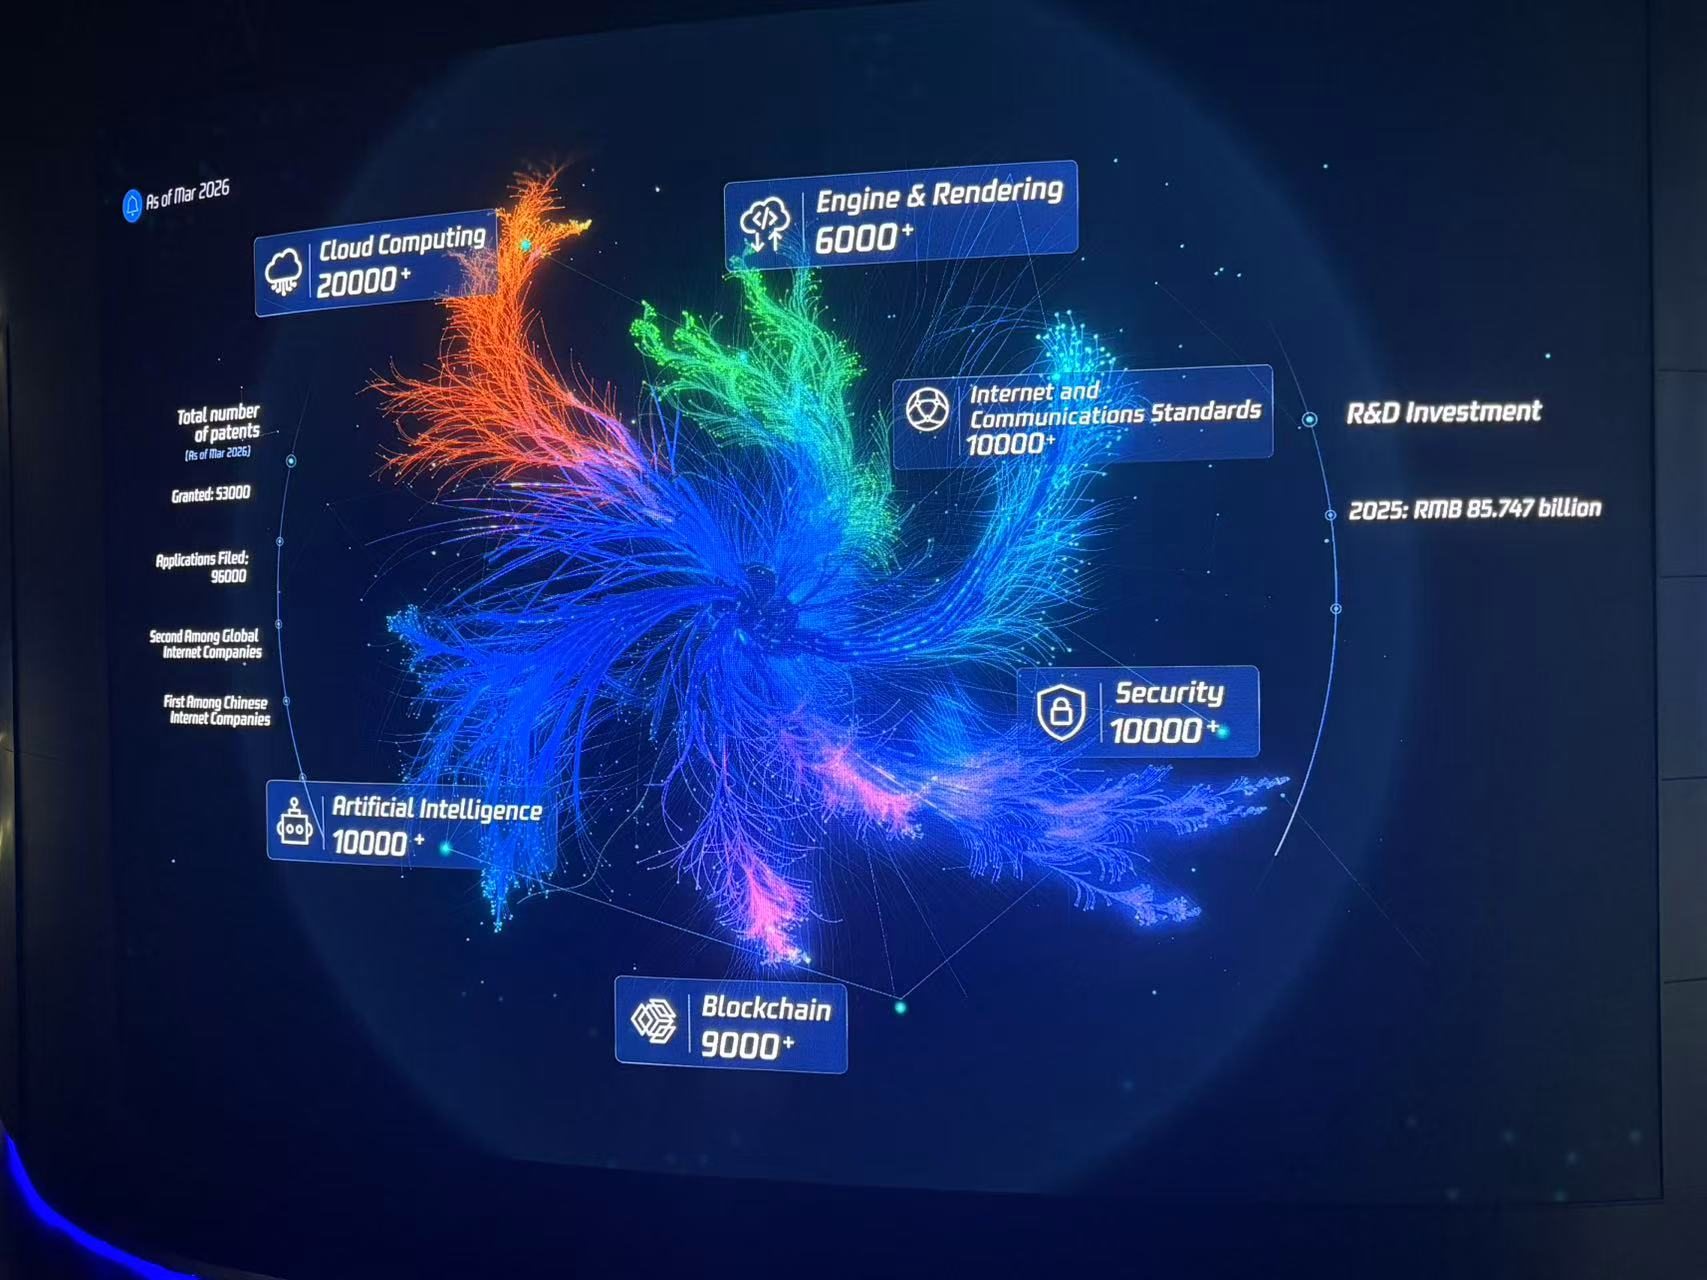
\includegraphics[width=\columnwidth]{figures/tencent.jpg}
\caption{\normalfont Patent and R\&D display, \textbf{Tencent Shanghai Office}, September 4, 2026, photographed by the author. \textbf{Observation:} six labelled patent categories, Security among them at 10000+, with 53000 granted patents and 2025 R\&D investment of RMB 85.747 billion, as displayed on the day and not independently verified. \textbf{Interpretation:} protection is measured in inputs, not in outcomes for victims. \textbf{Relevance:} motivates the indexing question in Section~1.}
\Description{A dark wall screen showing a radial burst of coloured filaments surrounded by labelled boxes naming six patent categories.}
\label{fig:tencent}
\end{figure}

\begin{figure}[h]
\centering
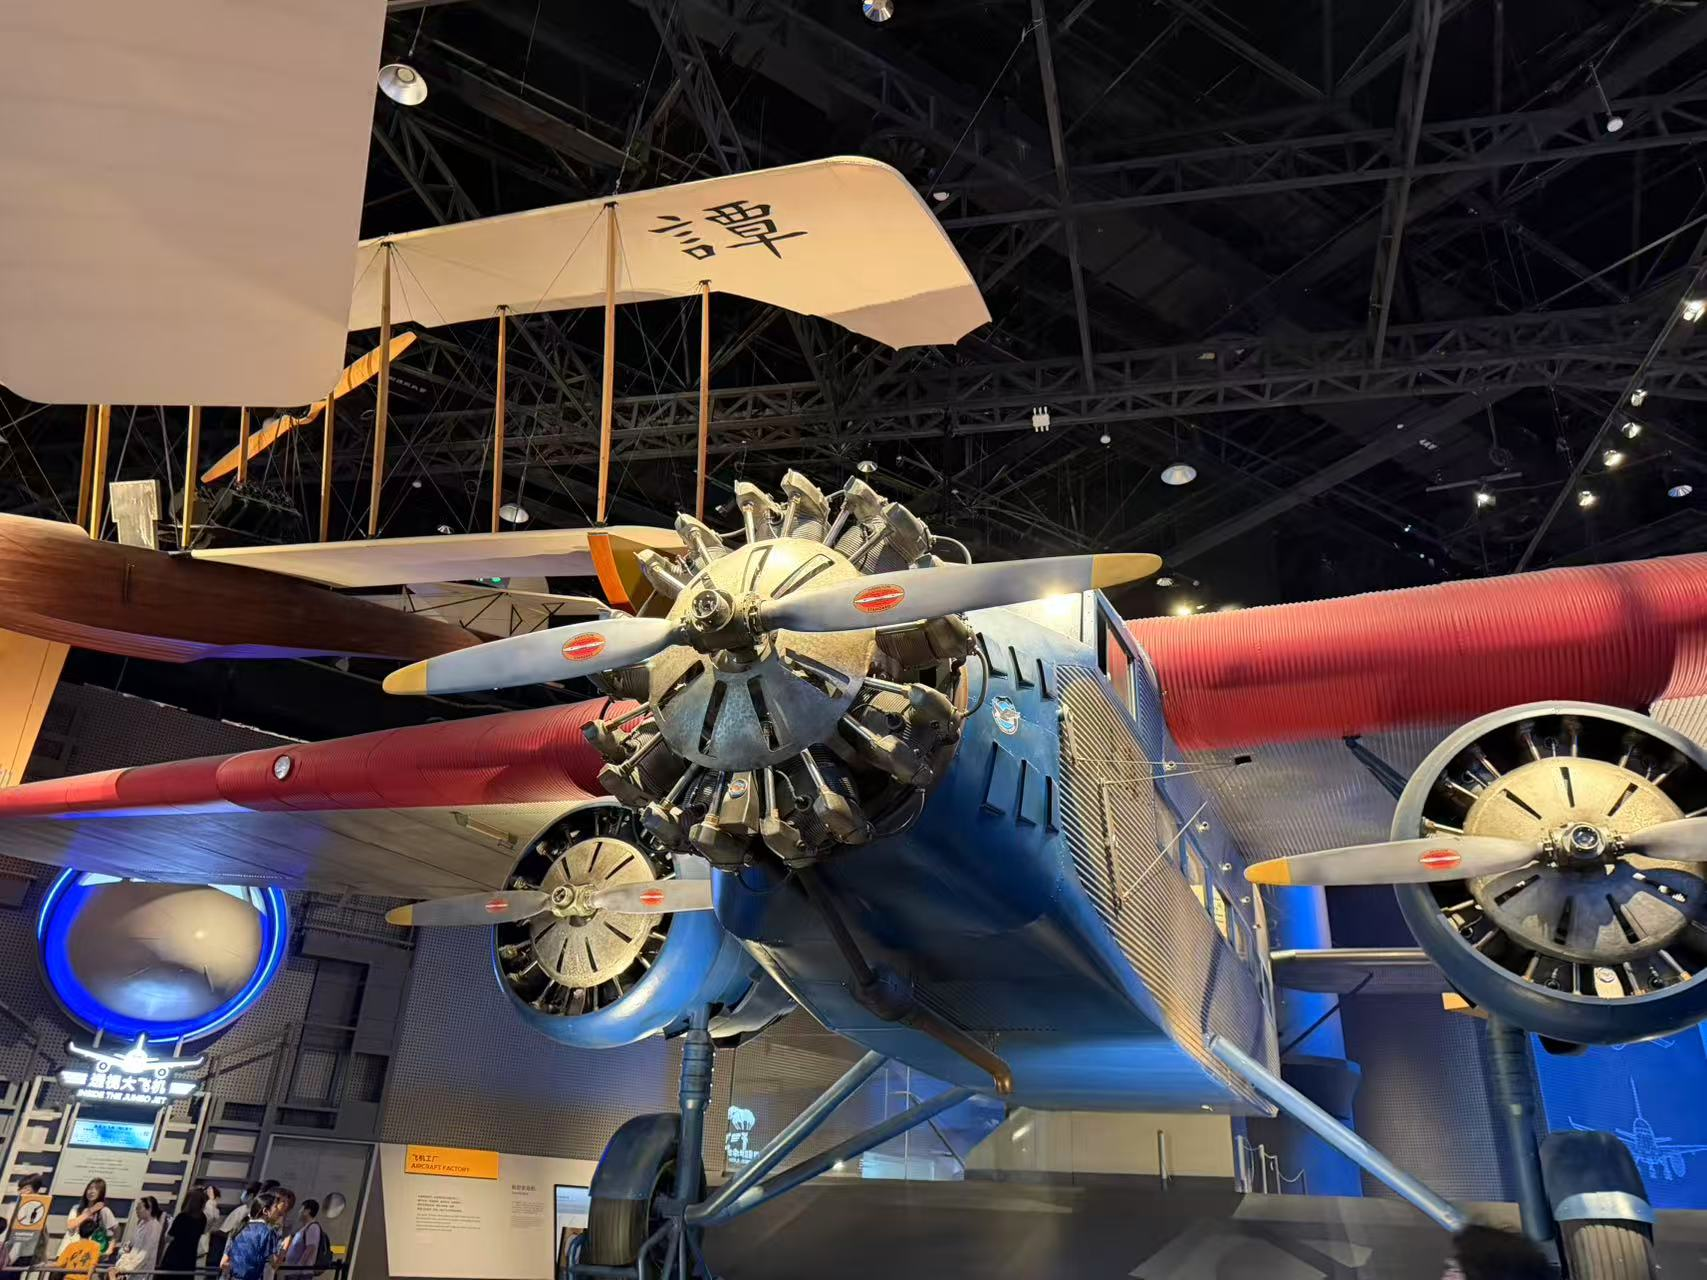
\includegraphics[width=\columnwidth]{figures/museum.jpg}
\caption{\normalfont Aviation gallery, \textbf{Shanghai Science and Technology Museum}, September 4, 2026, photographed by the author. \textbf{Observation:} two eras of airframe in one sightline, labelled by factory and interior. \textbf{Interpretation:} the exhibit makes the system, not the operator's judgement, the object to be understood. \textbf{Relevance:} public institutions can make pooled reporting compulsory, which is what lifts the reporting rate in Section~3.}
\Description{A trimotor aircraft beneath a suspended early biplane, with an orange exhibit label reading AIRCRAFT FACTORY.}
\label{fig:museum}
\end{figure}

\textbf{Private-sector value.} The platform alone sees both the customer's session and the payee's history, yet on an input-based measure adding detectors is countable while sharing payee records is a net private loss. The obstacle is the unit of account, not capability.

\textbf{Public-sector value.} Aviation safety came from mandatory pooled reporting, cross-carrier aggregation and certification rather than from questioning operators. Only public institutions can make such pooling compulsory---the step that lifts participation past its volunteer ceiling.

\textbf{Open-source inspiration.} Neither tool's licence matches its repository label, and they fail in opposite directions, which is why both licences were read in full rather than taken from the repository page.

\begin{itemize}
\item \textbf{OpenCTI} (Filigran). Official page \url{https://opencti.io}; source \url{https://github.com/OpenCTI-Platform/opencti}; version 7.260619.0; accessed September 6, 2026. A single LICENSE file governs both an Apache-2.0 Community Edition and a proprietary Enterprise Edition. \emph{Capability:} pools threat intelligence across institutions under the STIX2 standard. \emph{Limitation:} it shares indicators rather than account-level records, and participation is voluntary, so coverage is an institutional variable rather than a software one; default telemetry and map-server IP logging also show how shared infrastructure accretes secondary purposes. \emph{Design consequence:} the cross-institution reporting rate is a parameter in my game rather than a constant, and $p=0$ is reported as a boundary case.

\item \textbf{FairGBM} (Feedzai). Source \url{https://github.com/feedzai/fairgbm}; version 0.9.14; accessed September 6, 2026. GitHub labels the repository ``Other'' and the README asks commercial users to make contact, but the LICENSE is Apache 2.0 concatenated with upstream LightGBM's MIT, both of which permit commercial use without prior consent. \emph{Capability:} imposes group error-rate constraints during gradient boosting for fraud settings. \emph{Limitation:} it constrains error rates given the input features, so it cannot recover a signal the adversary authored. \emph{Design consequence:} it separates two failure channels---who bears misclassification cost, and who wrote the signal being classified---and supplies the published group false-flag rate that Section~5 requires as a governance condition.
\end{itemize}

\section{Review response and revision record}
\label{app:review}
Peer review is scheduled for September 14, 2026 and has not yet taken place, so this appendix is pending. It will retain v1, both peer reviews, my author response, reviewer follow-up and v2, organised by the three review themes: strengths to retain, constructive concerns to address, and questions to clarify. Each response will name the change, its location and the verification actually performed, or justify retaining the approach or deferring the work.

\textbf{Submission milestones.} First draft September 13, 2026, 11:00 P.M. Beijing time (UTC+8); class review September 14; proposed rebuttal September 16 and revised submission September 20, both at 11:00 P.M.

\clearpage\onecolumn
\section{Structured abstract and cumulative proposal map}\label{app:abstract}
The eight rows below are the current version. The Intellectual Statement II version is preserved in the repository history at an earlier commit. The first seven rows summarise the research; the last records feedback and revision.
\par\medskip
\begin{table}[H]
\caption{Appendix E structured abstract; the eight-row proposal structure is retained.}
\label{tab:abstract-map}
\renewcommand{\arraystretch}{1.18}
\begin{tabularx}{\textwidth}{@{}p{0.27\textwidth}Y@{}}
\toprule
\textbf{Proposal element} & \textbf{Current statement / change} \\
\midrule
Background & Cooperation survives on minimal information, but the cited results assume an authentic signal. Authorised push payment fraud breaks this: \pounds576.4 million lost across 248,070 cases in 2025, with split reimbursement required since 2024. Key foundation: mechanism design (Hurwicz, Maskin and Myerson, Nobel 2007). \\
Motivation and application & The reporting channel is authored by the adversary, so deception cues are absent and a paid check returns his text. Scenario: retail payment verification, generalising to reputation systems in which a rated party writes its own signal. Affected: payers and payees least able to document themselves. \\
Three connected questions & Economics: how should a depleting verification budget be allocated? Computation: which mechanisms are coaching-proof against an adversary that adapts? Behavior: is decay or authorship the binding constraint? Integrated: the budget is scarce, depletes and must be recomputed, so all three are required at once. \\
Method and model assumptions & Players: fraudster, bank, regulator. The bank selects a mechanism rather than a verdict per episode; information is incomplete in Harsanyi's sense; solution concept Bayesian Nash equilibrium. Baseline: a seeded client-side simulation in which the fraudster best-responds between rounds. Evidence needed: a sweep of the reporting rate and an ablation of habituation. \\
Results or expected results & Obtained (simulated): the miss rate tracks $1-p$ to within 0.032; the habituation gap is 0.401 at script rate 0 and 0.000 at script rate 1; the notebook reproduces three payoffs recorded in the deployed game exactly. Expected, not obtained: on real payment data, payee-indexed checking blocks fewer legitimate transactions at equal interception. A testimony-based mechanism invariant to a passing script would challenge the claim. \\
Intellectual merits & Habituation becomes a mechanism's state variable rather than an interface problem; costly verification is extended to checks that return the adversary's text; history-dependent cost defeats static tractability. Together they explain why mandated warnings keep expanding after being shown ineffective. \\
Practical impacts & Private: reallocate warning spend rather than increase it, since the platform alone holds both signals. Public: coaching-proofness can replace ``was a warning issued?'' as the compliance test. SDG 4: the open-access game teaches why authorship determines a mechanism's effectiveness; usefulness assessed by the change in correct justifications before and after play, not correct guesses. \\
Feedback received and revision made & Field evidence, Tencent Shanghai Office, September 4, 2026: protection is counted in inputs. I previously asked how much friction to spend; I changed the question to what friction is indexed to (Sections 1 and 5). Session D discussion, September 7, 2026, moved the criterion from payments to reputation systems generally. Peer review is pending as of September 13, 2026. \\
\bottomrule
\end{tabularx}
\end{table}
\noindent Field observations, photographs, open-source inspirations and the AI-use disclosure are in Appendices~\ref{app:tech}--\ref{app:field}. Observation, interpretation and proposed future evidence are distinguished throughout. The Open Science Statement groups GitHub and Colab; the Statement of Contribution to the UN's SDGs groups the Hugging Face learning tool.